\documentclass[./main.tex]{subfiles}

\begin{document}
\section{Deep Learning Theory}
The following section covers the most important background theory for the experiments in Section \ref{sec:experiments}. This includes an introduction to various types of neural networks, as well as an introduction to the optimization of such networks.

\subsection{Feedforward Neural Networks}
\textbf{Feedforward neural networks} are the most basic type of neural networks. The aim of a feedforward neural network is to approximate some function $f^*$, by defining a mapping $\bm{y} = f(\bm{x}; \bm{\theta})$ and learning the parameters $\bm{\theta}$, that results in the best approximation of $f^*$. These models are called \textbf{feedforward} because there are no \textbf{feedback} connections in which the outputs of the model are fed back into itself. Instead, information flows through the function being evaluated from $\bm{x}$, through the intermediate computations used to define $f$, and finally to the output $\bm{y}$. Feedforward neural networks generally consists of multiple \textbf{layers}, arranged in a chain structure, with each layer being a function of the layer that preceded it \cite{DL_book}. 

\subsubsection{Fully-connected Layers}
The most simple type of layer found in a feeforward neural network is the \textbf{fully-connected layer}. The fully-connected layer usually consists of some learnable parameter matrix $\bm{W}$ and learnable parameter vector $\bm{b}$, as well as a non-linear \textbf{activation function} $g$ (which will be covered further in Section \ref{subsubsec:activation_func}). In this case, the $i$'th layer is defined as \cite{DL_book}
\begin{equation}
    \bm{h}^{(i)} =
    \begin{cases}
        g^{(i)} \left( \bm{W}^{(i) \top} \bm{h}^{(i)} + \bm{b}^{(i)} \right) & \text{if } i > 1 \\
        g^{(1)} \left( \bm{W}^{(1) \top} \bm{x} + \bm{b}^{(1)} \right) & \text{if } i = 1
    \end{cases}
    .
\end{equation}

\subsubsection{Convolutional Layer}
\begin{figure}[htbp]
    \centering
    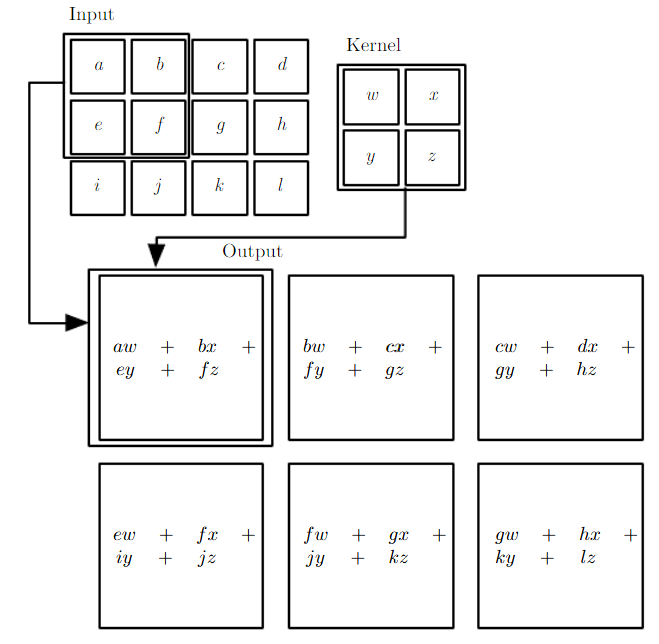
\includegraphics[width = 0.5 \textwidth]{./entities/2d_conv_example.PNG}
    \caption{An example of applying a 2d kernel on an input \cite{DL_book}.}
    \label{fig:2d_conv_example}
\end{figure}
\noindent A \textbf{convolutional layer} is a specialized kind of feedforward layer, usually used in analysis of time-series or image data \cite{DL_book}. If a network has at least one convolutional layer, it is called a \textbf{Convolutional neural network (CNN)}.
\\
\\
\noindent The convolutional layer consists of a set of \textbf{kernels}, each to be applied to the entire input vector, where each kernel is a learnable parameter matrix $k \times k$ \cite{everything}. Each kernel is applied on the input to produce a \textbf{feature map}. The kernels are applied to the input by "sliding" over the input (where the step size is called \textbf{stride}). Each $k \times k$ grid of the input is then used to compute the dot-product between the grid and each kernel, which is then placed in the corresponding feature map of each kernel, as visualized in Figure \ref{fig:2d_conv_example}. \cite{bsc_thesis}. To control the dimensions of the output, one might \textbf{pad} the sides with a constant value. Commonly, zero is used as the padding-value.
\\
\\
As seen in Figure \ref{fig:2d_conv_example}, each kernel produces a linear combination of all pixel values in a neighbourhood defined by the size of the kernel. Thus, unlike a fully-connected layer, a convolutional layer captures the high correlation between a pixel and its neighbours. Further, by limiting the size of the kernel, the network will use much fewer parameters, than if a fully-connected layer would be used instead \cite{DL_book}.

\subsection{Recurrent Neural Networks}
\begin{figure}[htbp]
    \centering
    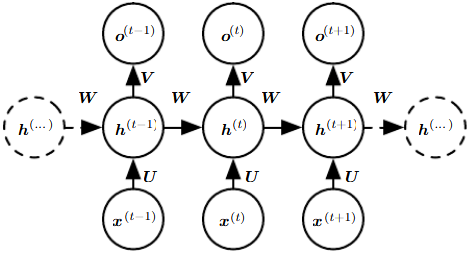
\includegraphics[width = 0.5 \textwidth]{./entities/rnn_illustration.PNG}
    \caption{An illustration of an RNN \cite{DL_book}.}
    \label{fig:rnn_illustration}
\end{figure}
\noindent \textbf{Recurrent neural networks (RNNs)} are a family of neural networks for processing sequential data. Figure \ref{fig:rnn_illustration} illustrates the general setup of such a network, which maps an input sequence of $\bm{x}$ values to a corresponding sequence of output $\bm{o}$ values. Generally, a RNN consists of three parts: (1) the input ($\bm{x}^{(i)}$), (2) the hidden state ($\bm{h}^{(i)}$), and (3) the output ($\bm{o}^{(i)}$). During inference, the model maps each input value to an out value, in a sequential matter, where it first maps the first input value, then the second, then the third, and so forth. The network maps each input value to an output value by making use of the hidden state from the preceding step, where the first hidden state has to be initiallized \cite{DL_book}.

\subsubsection{Convolutional Long Short-Term Memory}
One common recurrent neural network unit is the \textbf{convolutional long short-term memory (ConvLSTM) cell}, which is an adaptation of the standard \textbf{long short-term memory (LSTM) cell} for sequences of images. 
\\
\\
\noindent The idea of the ConvLSTM cell is to create paths through time that have derivatives that neither vanish nor explode. This is done by accumulating information over a long duration. Once that information has been used, the cell \textit{forgets} the old state, which the ConvLSTM cell learns to decide when to clear. Each cell has the same inputs and outputs as an ordinary reccurent network, but also has more parameters and a system of gating units that controls the flow of information \cite{DL_book}.
\\
\\
The ConvLSTM cell is defined as the following. Let $\bm{X}_1, \bm{X}_2, ..., \bm{X}_t$ be a sequence of input images, $\bm{C}_1, \bm{C}_2, ..., \bm{C}_t$ be a sequence of cell outputs, and $\bm{H}_1, \bm{H}_2, ..., \bm{H}_t$ be a sequence of hidden states. Then, at each input step $t$, we compute \cite{conv_lstm}
\begin{align}
    \bm{i_t} &= \sigma \left( \bm{W}_{xi} * \bm{X}_t + \bm{W}_{hi} * \bm{H}_{t - 1} + \bm{W}_{ci} \circ \bm{C}_{t - 1} + \bm{b}_i \right) \\
    \bm{f_t} &= \sigma \left( \bm{W}_{xf} * \bm{X}_t + \bm{W}_{hf} * \bm{H}_{t - 1} + \bm{W}_{cf} \circ \bm{C}_{t - 1} + \bm{b}_f \right) \\
    \bm{C}_t &= \bm{f}_t \circ \bm{C}_{t - 1} + \bm{i}_t \circ \text{tanh} \left( \bm{W}_{xc} * \bm{X}_t + \bm{W}_{hc} * \bm{H}_{t - 1} + \bm{b}_c \right) \\
    \bm{o}_t &= \sigma \left( \bm{W}_{xo} * \bm{X}_t + \bm{W}_{ho} * \bm{H}_{t - 1} + \bm{W}_{co} \circ \bm{C}_t + \bm{b}_\circ \right) \\
    \bm{H}_t &= \bm{o}_t \circ \text{tanh}(\bm{C}_t)
\end{align}

\subsubsection{Gated Recurrent Unit}


\subsection{Transformer}
\subsubsection{Encoder}
\subsubsection{Decoder}

\subsection{Training a Neural Network}
\subsubsection{Activation function}
\label{subsubsec:activation_func}

\end{document}